\section{Введение}

В данной главе рассматривается проблема моделирования физических систем, решение дифференциальных уравнений с применением нейронных сетей. В этой области имеется проблема: существующие подходы с нейронными сетями не имеют априорных знаний о физике. Это мешает им выучить точные физические законы. В главе рассмотрен один из подходов, как решать эту проблему: учить из данных законы сохранения/инвариантные величины на основе гамильтоновой или лагранжевой механики.

\section{Литература}

\begin{itemize}
	\item \textit{Greydanus et al.} Hamiltonian Neural Networks, // Advances in Neural Information Processing Systems, 2019
	\item \textit{M. Cranmer, Greydanus et al.} Lagrangian Neural Networks // arXiv preprint, 2020
	\item \textit{Greydanus et al.}  Blog post on Hamiltonian Neural Networks // \\https://greydanus.github.io/2019/05/15/hamiltonian-nns
	\item \textit{Greydanus et al.}  Blog post on Lagrangian Neural Networks article // \\https://greydanus.github.io/2020/03/10/lagrangian-nns
\end{itemize}


\section{Hamiltonian and Lagrangian Neural Networks}

Вспомним, как решается рассматриваемая задача в классических подходах теоретической механики. Рассмотрим подход с гамильтоновй механикой.

\subsection{Гамильтонова механика}
\begin{enumerate}
	\item Выбрать набор координат, описывающих состояние системы: $\textbf{q}=(q_1, \cdots,q_N)$ -- позиции, $\textbf{p}=(p_1,\cdots,p_N)$ -- импульсы.
	\item Записать полную энергию системы как функцию этих координат (гамильтониан $\mathcal{H}$). 
	\item Используя уравнения Гамильтона, найти производные системы по времени:
	$$
	\frac{d \mathbf{q}}{d t}=\frac{\partial \mathcal{H}}{\partial \mathbf{p}}, \quad \frac{d \mathbf{p}}{d t}=-\frac{\partial \mathcal{H}}{\partial \mathbf{q}}
	$$
	Получили эволюцию координат ($\textbf{q, p}$) по времени: $
	\mathbf{S}_{\mathcal{H}}=\left(\frac{\partial \mathcal{H}}{\partial \mathbf{p}},-\frac{\partial \mathcal{H}}{\partial \mathbf{q}}\right)
	$
	\item Интегрировать полученные производные по времени для получения состояния системы в какой-то момент времени в будущем: $$ \left(\mathbf{q}_{1}, \mathbf{p}_{1}\right)=\left(\mathbf{q}_{0}, \mathbf{p}_{0}\right)+\int_{t_{0}}^{t_{1}} \mathbf{S}(\mathbf{q}, \mathbf{p}) d t$$
	
\end{enumerate}

На основе этой последовательности действий строится Гамильтонова нейронная сеть:


\subsection{Hamiltonian Neural Networks}

\begin{itemize}
	\item \textbf{Ключевая идея}: параметризовать нейронной сетью гамильтониан $\mathcal{H}$, а не  $\frac{\Delta \mathbf{q}}{\Delta t},  \frac{\Delta \mathbf{p}}{\Delta t}$
	\item \textbf{Задача оптимизации} из уравнений Гамильтона: 
	$$
	\underset{\theta}{\operatorname{argmin}}\left\|\frac{d \mathbf{q}}{d t}-\frac{\partial \mathcal{H}_{\theta}}{\partial \mathbf{p}}\right\|^{2}+\left\|\frac{d \mathbf{p}}{d t}+\frac{\partial \mathcal{H}_{\theta}}{\partial \mathbf{q}}\right\|^{2}
	\Rightarrow $$
	
	$$\Rightarrow \mathcal{L}_{H N N}=\left\|\frac{\partial \mathcal{H}_{\theta}}{\partial \mathbf{p}}-\frac{\partial \mathbf{q}}{\partial t}\right\|_{2}+\left\|\frac{\partial \mathcal{H}_{\theta}}{\partial \mathbf{q}}+\frac{\partial \mathbf{p}}{\partial t}\right\|_{2}
	$$
\end{itemize}

Наглядно отличие от классического подхода с нейронными сетями можно увидеть на \ref{hnn}.

\begin{figure}[h]
	\centering
	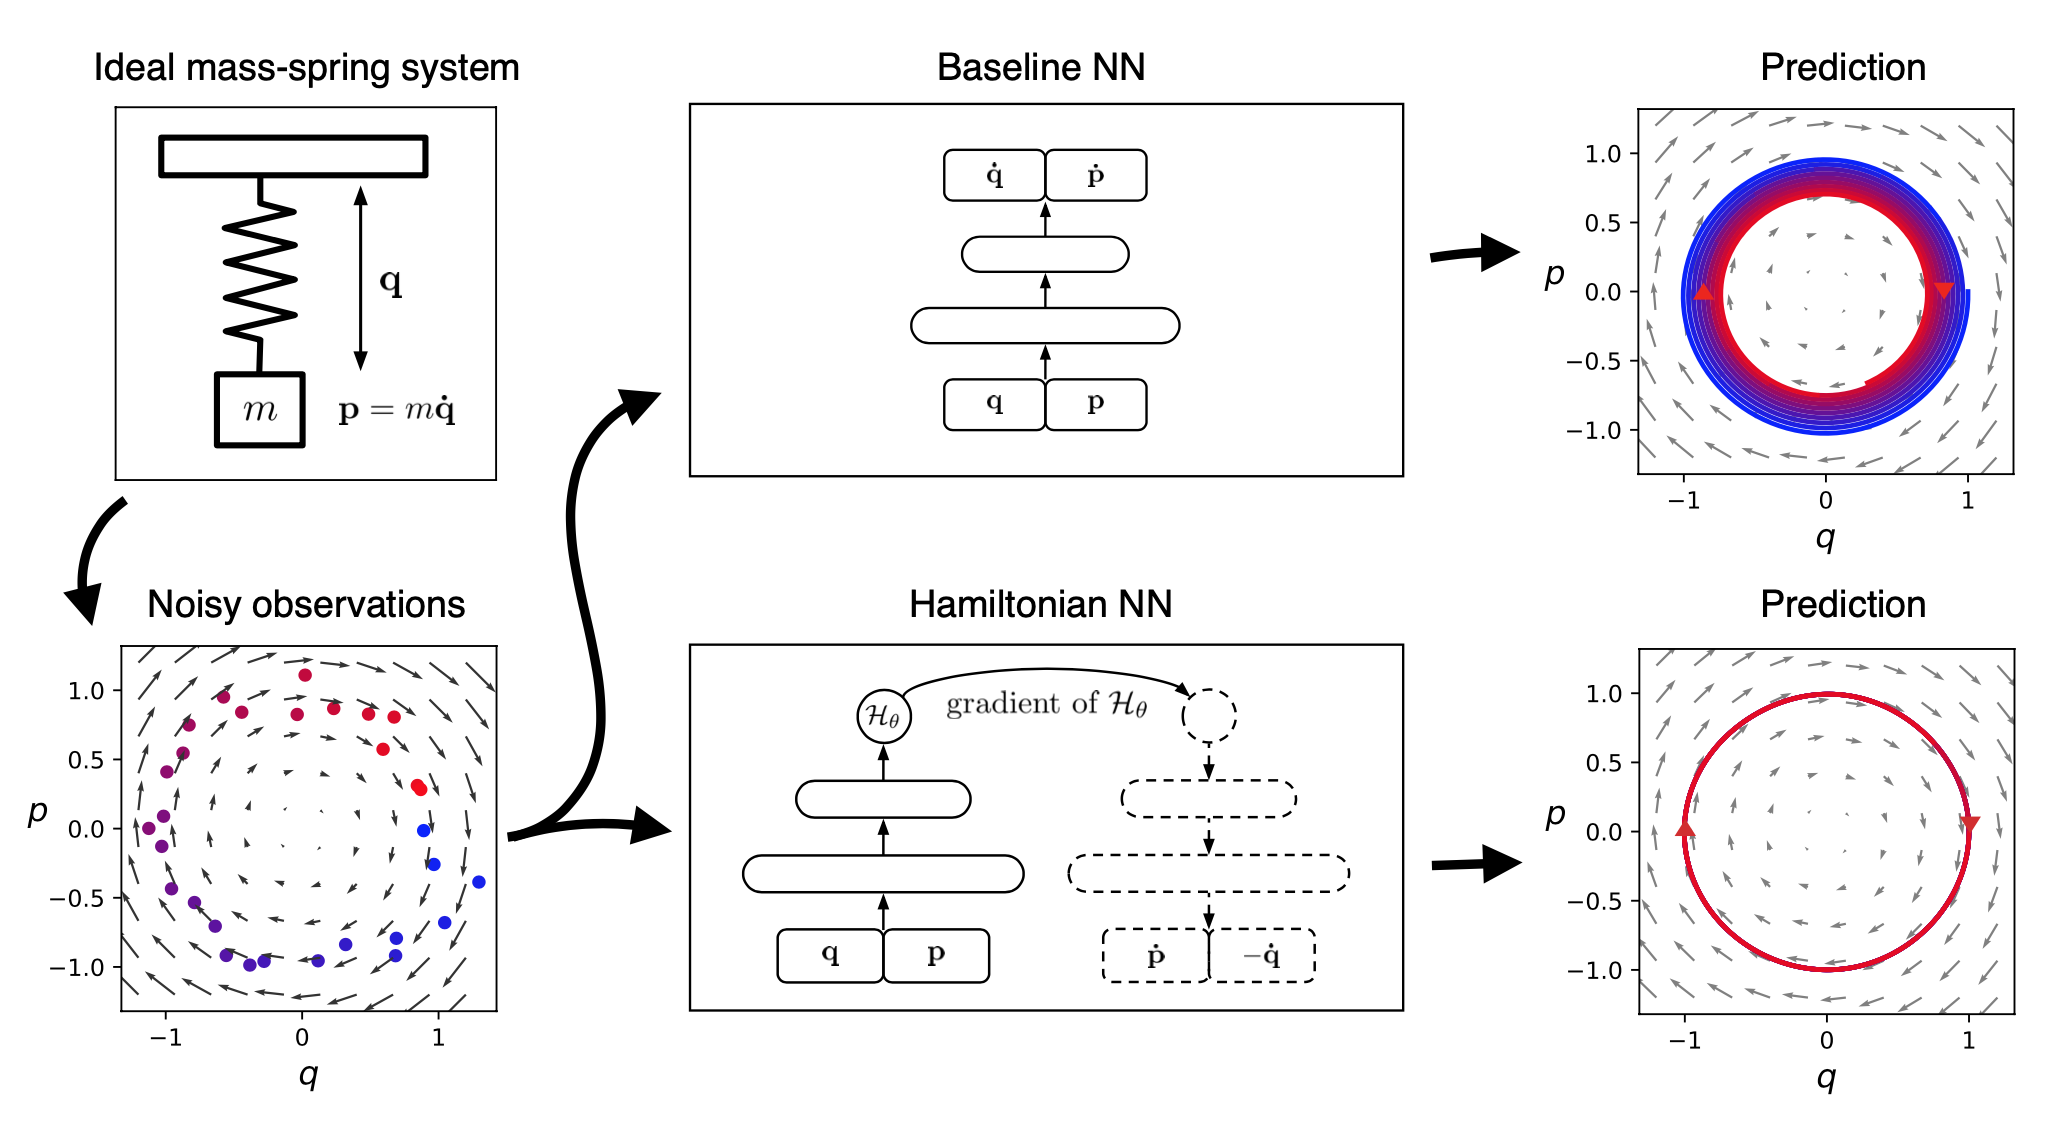
\includegraphics[width=0.99\textwidth]{hnn.png}
	\label{hnn}
	\caption{Рис.  Схема работы Hamiltonian Neural Networks (HNN) на системе с гамильтонианом $
		\mathcal{H}=\frac{1}{2} k q^{2}+\frac{p^{2}}{2 m} $ в сравнении с базовым решением (Baseline NN)}
\end{figure}

\begin{figure}[h]
	\centering
	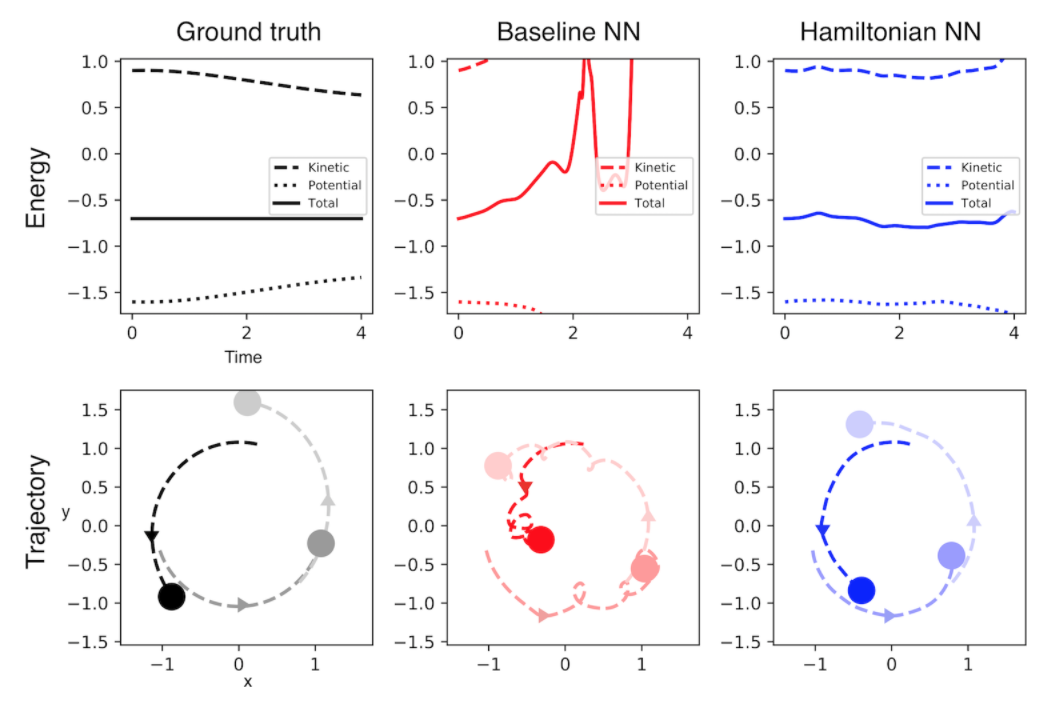
\includegraphics[width=0.89\textwidth]{3body_hnn.png}
	\label{3body_hnn}
	\caption{Рис. Взаимодействие трех тел посредством гравитационных сил. HNN превосходит по качеству решение без априорного знаниия о физике системы (Baseline NN)}
\end{figure}

На рисунке \ref{3body_hnn} представлен эксперимент моделирования задачи трех тел.

\subsection{Лагранжева механика}
\begin{itemize}
	\item \textbf{Проблемы HNN}: гамильтонов формализм требует, чтобы координаты системы были «каноническими»($(\textbf{q, p})$ должны подчиняться соотношениям, заданным скобками Пуассона) -- многие системы не удовлетворяют этому ограничению (часто $p \neq q \cdot m$)
	\item \textbf{Решение проблемы}: использовать лагранжианы систем (обеспечивают сохранение полной энергии, могут делать это с использованием произвольных координат)
\end{itemize}

Вспомним, как моделируется динамика системы с помощью лагранжиана:
\begin{enumerate}
	\item Найти аналитические выражения для кинетической и потенциальной энергии $(T, V )$
	\item Записать лагранжиан $\mathcal{L} = T - V $
	\item Применить ограничение Эйлера-Лагранжа $\frac{d}{d t} \frac{\partial \mathcal{L}}{\partial \dot{q}_{j}} =\frac{\partial \mathcal{L}}{\partial q_{j}} $
	\item Решить получившуюся систему дифференциальных уравнений
\end{enumerate}

\subsection{Lagrangian Neural Networks}

\begin{itemize}
	\item \textbf{Ключевая идея}: параметризовать нейронной сетью лагранжиан $\mathcal{L}$, получить выражение ограничения Эйлера-Лагранжа, обратно распространить ошибку через полученные ограничения
	\item Получение из параметризованного лагранжиана требуемых величин	$$
	\begin{aligned}
	\frac{d}{d t} \frac{\partial \mathcal{L}}{\partial \dot{q}_{j}} =\frac{\partial \mathcal{L}}{\partial q_{j}}  \Rightarrow \frac{d}{d t} \nabla_{\dot{q}} \mathcal{L} =\nabla_{q} \mathcal{L} \\
	\left(\nabla_{\dot{q}} \nabla_{\dot{q}}^{\top} \mathcal{L}\right) \ddot{q}+\left(\nabla_{q} \nabla_{\dot{q}}^{\top} \mathcal{L}\right) \dot{q} =\nabla_{q} \mathcal{L} \\
	\ddot{q} =\left(\nabla_{\dot{q}} \nabla_{\dot{q}}^{\top} \mathcal{L}\right)^{-1}\left[\nabla_{q} \mathcal{L}-\left(\nabla_{q} \nabla_{\dot{q}}^{\top} \mathcal{L}\right) \dot{q}\right]
	\end{aligned}
	$$
	\item Для заданного набора координат $x_t = (q_t, \dot{q}_t)$ получили метод вычисления $\dot{x}_t = (\dot{q}_t, \ddot{q}_t)$ из параметризованного лагранжиана.
	\item \textbf{Функция ошибки}: $$\mathcal{L} = \left\|\dot{x}^{\mathcal{L_{\theta}}}_t -\dot{x}^{true}_t\right\|_{2}$$
\end{itemize}

\begin{figure}[h]
	\centering
	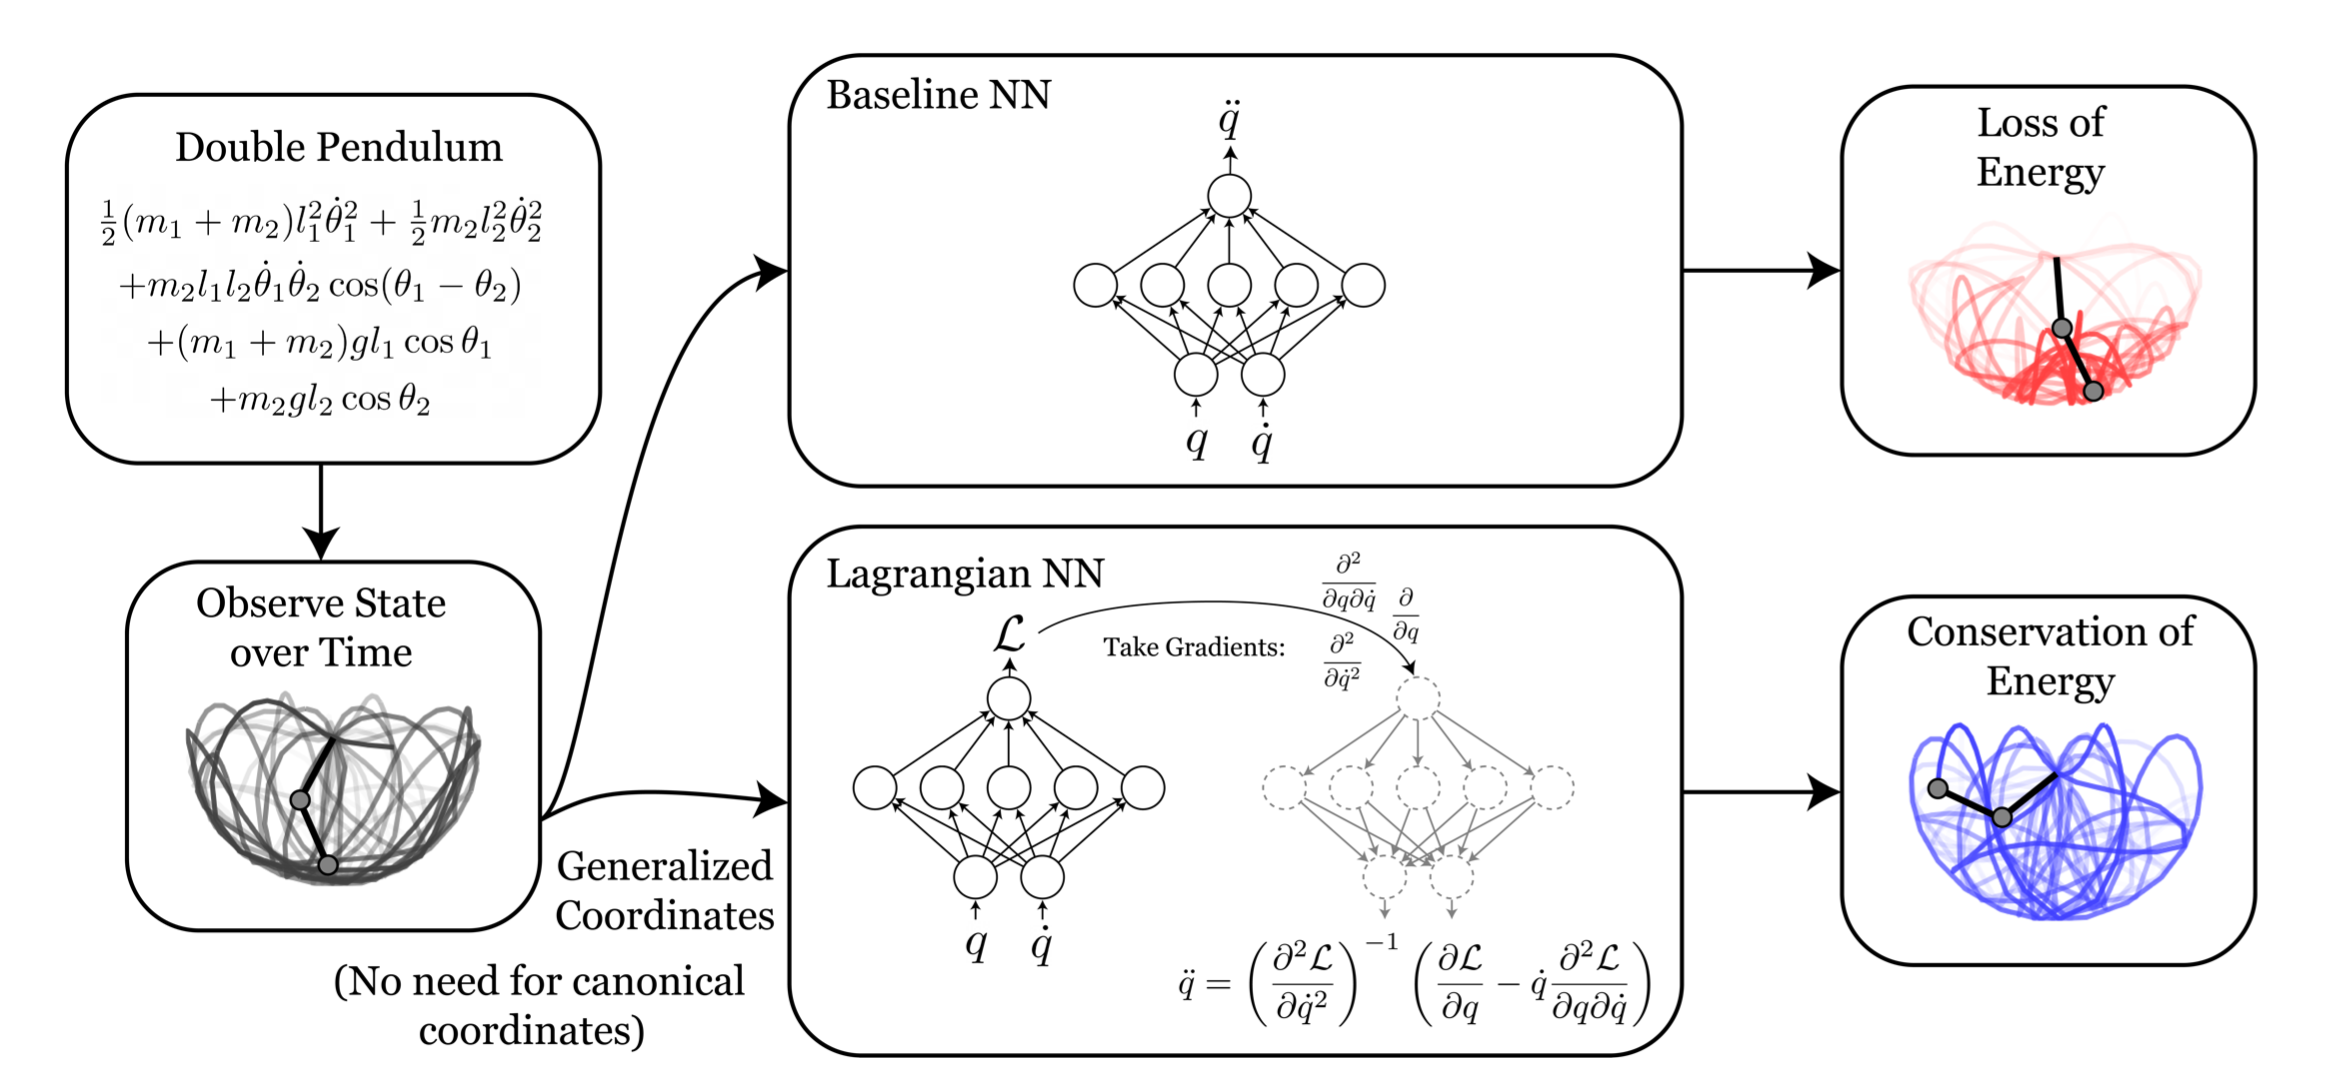
\includegraphics[width=0.9\textwidth]{lnn.png}
	\caption{Рис. Схема работы Lagrangian Neural Networks (LNN) моделирования динамики двойного маятника в сравнении с базовым решением (Baseline NN)}
\end{figure}

\subsection{Вычислительный эксперимент -- сравнение LNN и HNN}
Рассматривается частица с массой $m=1$, релятивистской скоростью $c=1$, движущейся в потенциале $g$. Лагранжиан системы: 
$$\mathcal{L}=\left(\left(1-\dot{q}^{2}\right)^{-1 / 2}-1\right)+g q$$
На рисунке \ref{hnn_vs_lnn} представлены эксперименты на рассматриваемой системе. В (а) модель HNN не может выучить динамику из неканонических координат. В (b) HNN удается выучить динамику, если заданы канонические координаты. В (c) LNN выучивает точную динамику из неканонических координат
\begin{figure}[h]
	\centering
	\label{hnn_vs_lnn}
	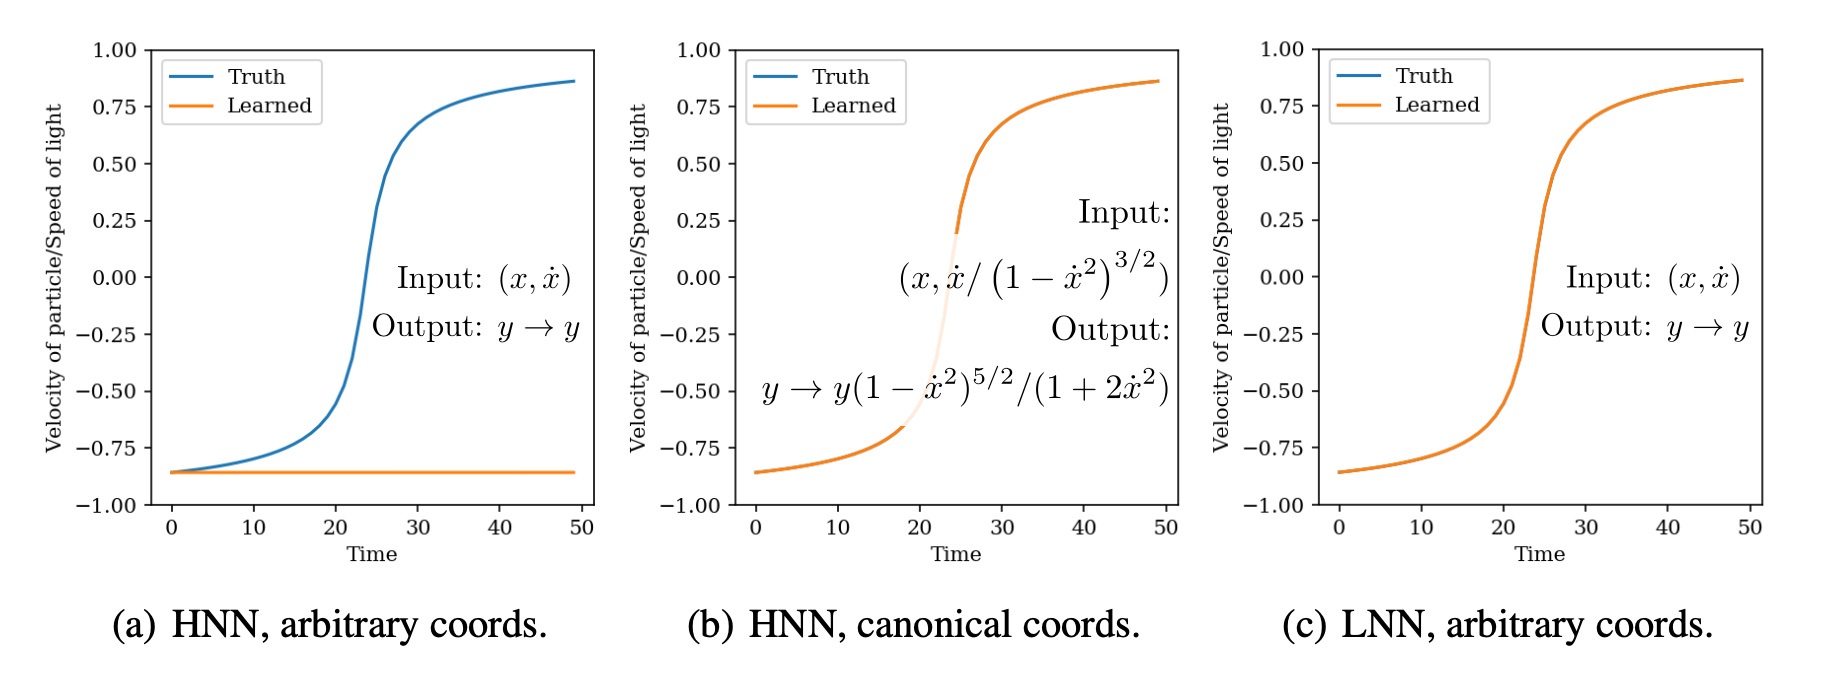
\includegraphics[width=0.8\textwidth]{hnn_vs_lnn.png}
	\caption{Рис. Результаты по задаче релятивистской частицы}
\end{figure}	
\newpage
\subsection{Сравнение подходов}
На \ref{comparison} представлено сравнение подходов HNN и LNN с классическим подходом, Neural ODE и DeLan.
\begin{figure}[h]
	\centering
	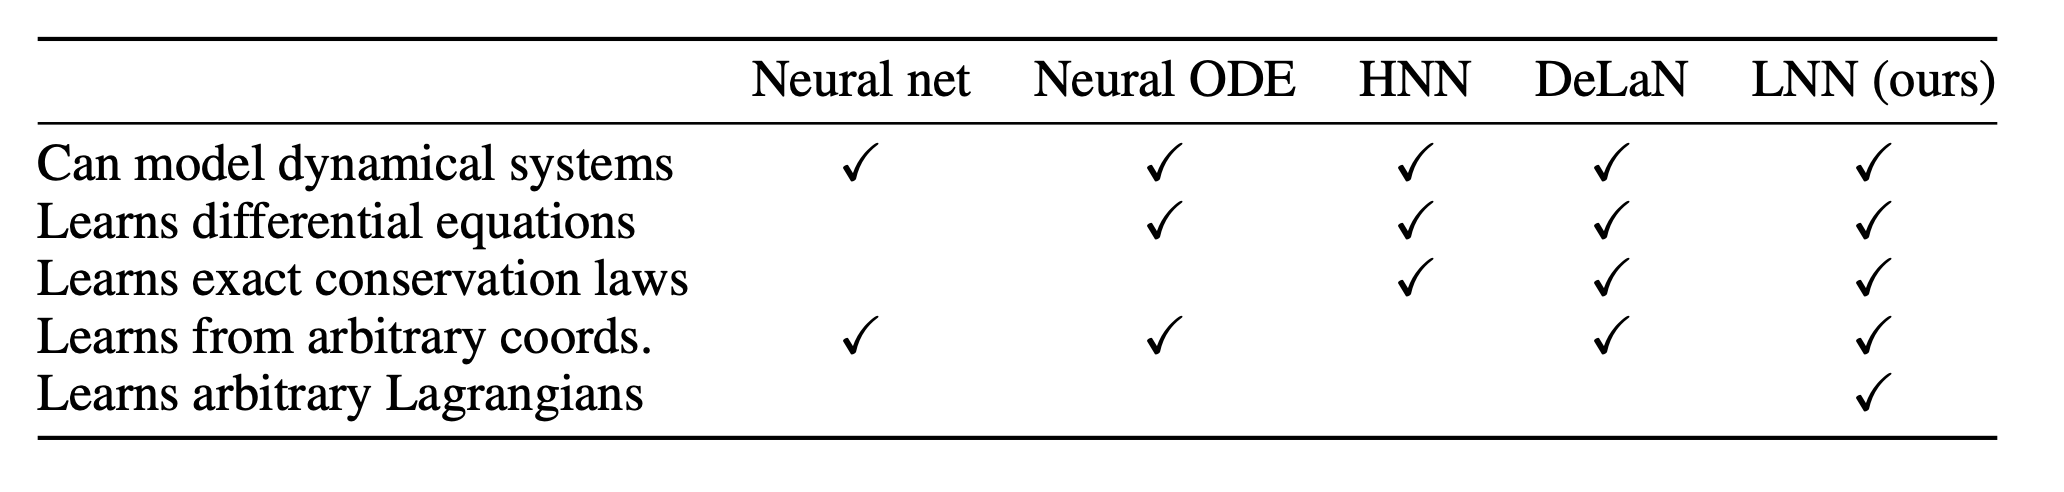
\includegraphics[width=0.9\textwidth]{comparison.png}
	\label{comparison}
	\caption{Рис. Сравнение подходов моделирования физических систем нейронными сетями}
\end{figure}


\section{Вопросы на обсуждение}

\begin{itemize}
	\item В чем мотивация рассмотренных моделей HNN и LNN?
	\item Что аппроксимирует нейронная сеть в HNN, в LNN?
	\item В чем преимущество LNN над HNN? 
\end{itemize}